
\begin{frame}
  \frametitle{Improving performance}
  \framesubtitle{Leaf node capacity}

  {\color{white} 
    \begin{center}
      \begin{tikzpicture}
        \centering
        \begin{axis}[
            every axis plot post/.style={/pgf/number format/fixed},
            axis on top,
            xtick=data,
            width=0.9\textwidth,
            height=6cm,
            enlarge x limits=0.2,
            symbolic x coords ={10, 20, 30, 40, 50, 60, 70, 80},
            axis lines*=left, 
            clip=false,
            title = Leaf capacity vs Pointer Dereferences,
            xlabel = Leaf Node Capacity,
            ylabel = Pointer Dereferences,
            ymajorgrids,
            major grid style = {dashed,white!50!gray},
            legend style = {fill=seashell-bg,draw=white}
          ]

          % BF = 8
          \addplot[graph-green] coordinates {(10,49) (20, 40) (30, 35) (40, 33) 
          (50, 26) (60, 23) (70, 21) (80, 22)};

          % BF = 16
          \addplot[graph-red] coordinates {(10,41) (20, 34) (30, 31) (40, 29) 
          (50, 27) (60, 25) (70, 24) (80, 25)};

          % BF = 32
          \addplot[graph-yellow] coordinates {(10,50) (20, 38) (30, 23) (40, 20) 
          (50, 19) (60, 18) (70, 18) (80, 19)};

          % BF = 64
          \addplot[graph-blue] coordinates {(10,32) (20, 26) (30, 23) (40, 22) 
          (50, 20) (60, 20) (70, 18) (80, 19)};

          \legend{8, 16, 32, 64}

        \end{axis}
      \end{tikzpicture}
    \end{center}
  }

\end{frame}

\begin{frame}
  \frametitle{Improving performance}
  \framesubtitle{Path selection}

  \begin{columns}[T]
    \begin{column}{.4\textwidth}
      \begin{block}{}%
        {\color{white} To minimize pointer dereferences need to optimally %
        traverse nodes in tree}
      \end{block}
    \end{column}
    \begin{column}{.6\textwidth}
      \begin{block}{}
        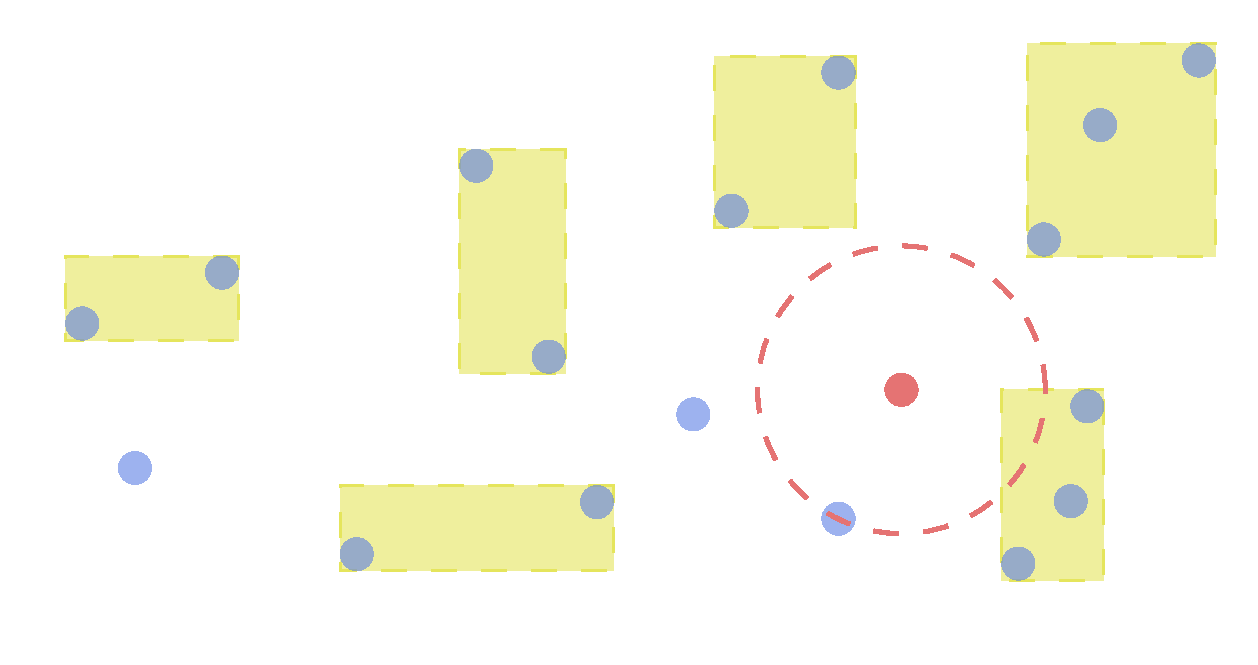
\includegraphics[width=\textwidth]{nn_adjaceny_complex_bound.pdf}
      \end{block}
    \end{column}
  \end{columns}

\end{frame}

\begin{frame}
  \frametitle{Improving performance}
  \framesubtitle{Path selection}

  \begin{figure}
    \centering
    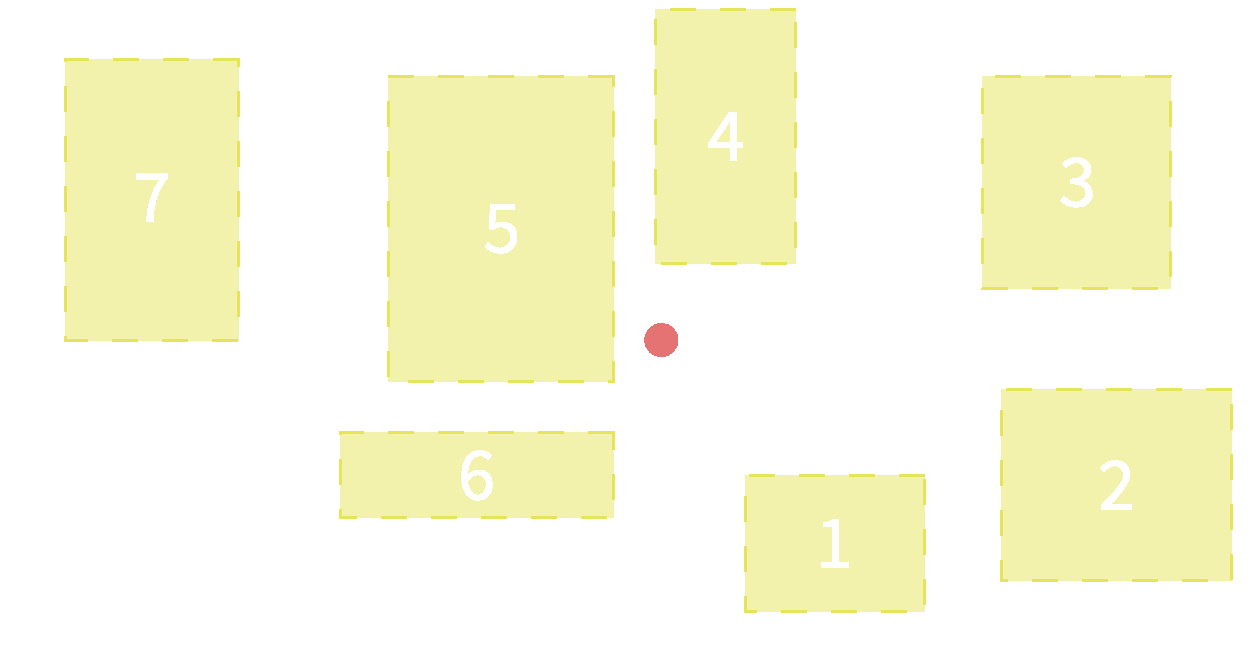
\includegraphics[width=0.85\textwidth]{nn_path_bad.pdf}
  \end{figure}

\end{frame}

\begin{frame}
  \frametitle{Improving performance}
  \framesubtitle{Path selection}

  \begin{figure}
    \centering
    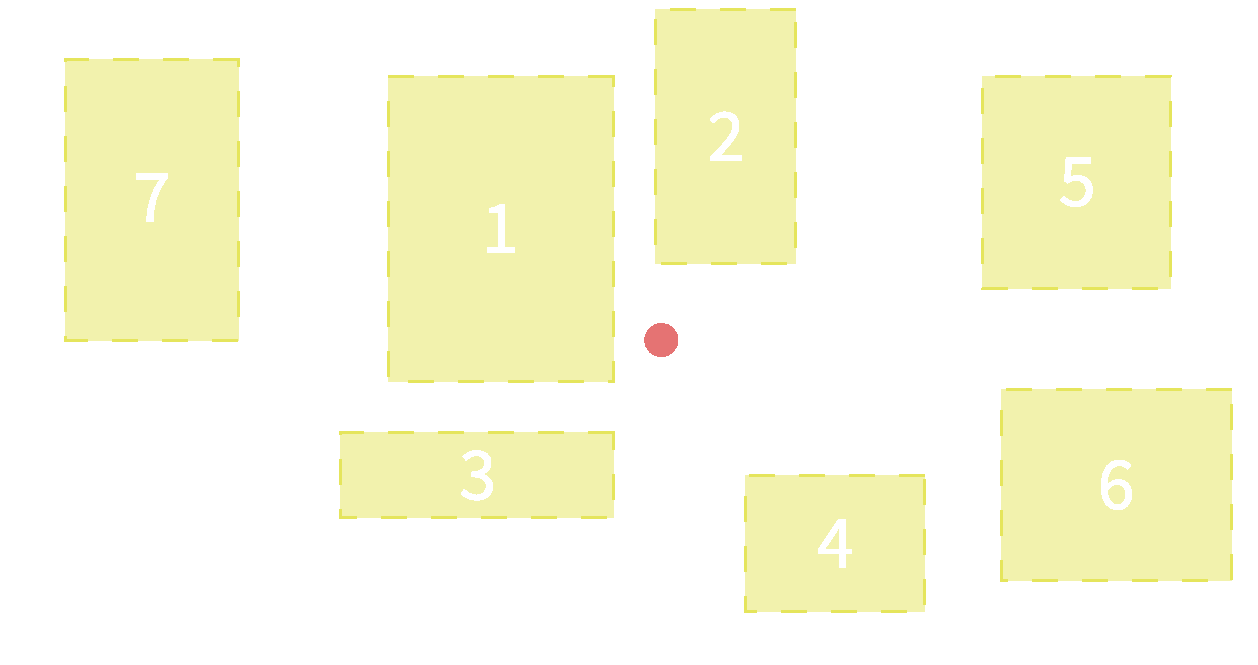
\includegraphics[width=0.85\textwidth]{nn_path_good.pdf}
  \end{figure}

\end{frame}

\begin{frame}
  \frametitle{Improving performance}
  \framesubtitle{Memory management}

  \begin{itemize}
    \item Many modern CPUs have cache line size of 64 bytes
      \begin{itemize}
        \item Size of double is 8 bytes, size of point is 24 bytes
      \end{itemize}
    \item Array of structs memory layout hampers SIMD performance 
  \end{itemize}

\end{frame}

\begin{frame}
  \frametitle{Improving performance}
  \framesubtitle{Memory management}

  \begin{figure}
    \centering
    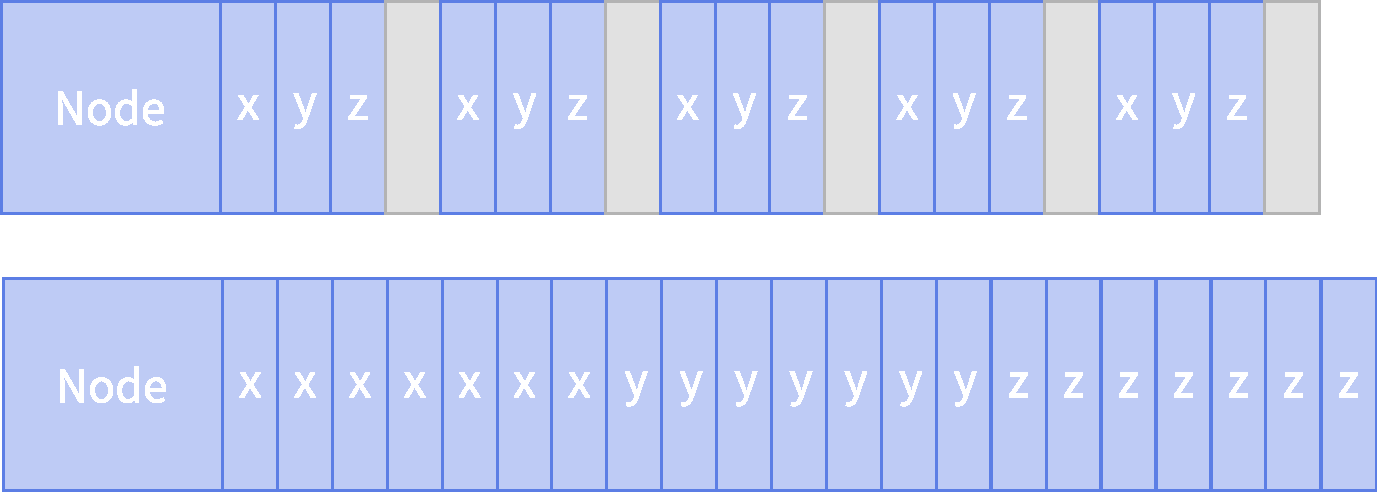
\includegraphics[width=0.85\textwidth]{memory.pdf}
  \end{figure}

\end{frame}
